\documentclass[border=1cm]{standalone}
\usepackage{tikz}
\usepackage{pgfplots}
\pgfplotsset{compat=1.12}

\usetikzlibrary{calc}
\usetikzlibrary{shapes.multipart}
\usetikzlibrary{positioning}

\tikzstyle{edge} = [draw, thick, shorten >=2pt, shorten <=2pt]
\tikzstyle{directed} = [edge, arrows={-latex}, shorten >=2pt, shorten <=0pt]
\tikzstyle{marked} = [tumred]
\tikzstyle{marked edge} = [very thick, marked]
\tikzstyle{marked node} = [very thick, draw=tumred, fill=tumred!15]
\tikzstyle{every text node part} = [align=center, execute at begin node=\setlength{\baselineskip}{2ex}]

%%%%%%%%%%%%
%  Locale  %
%%%%%%%%%%%%
\usepackage[english]{babel}
\selectlanguage{english}
\usepackage[T1]{fontenc}
\usepackage[utf8]{inputenc}

%%%%%%%%%%%
%  Fonts  %
%%%%%%%%%%%
\usepackage{textcomp}
\usepackage[sc,osf]{mathpazo}
% For scales see http://tex.stackexchange.com/a/2506
\usepackage[scaled=0.86]{berasans}
\usepackage[scaled=1.03]{inconsolata}
\linespread{1.05}
\usepackage{microtype}

%%%%%%%%%%%
%  Stuff  %
%%%%%%%%%%%
\usepackage{amsmath}

%%%%%%%%%%%%
%  Colors  %
%%%%%%%%%%%%
% Base Colors Corporate Design
\definecolor{tumblue}{HTML}{0065BD}
\definecolor{tumgreen}{HTML}{A2AD00}
\definecolor{tumorange}{HTML}{E37222}
\definecolor{tumivory}{HTML}{DAD7CB}
\definecolor{tumred}{HTML}{E53418} % not in Styleguide

% Derived Colors
% https://kuler.adobe.com/create/color-wheel/
% https://portal.mytum.de/corporatedesign/print/styleguide/
% Grays - TUM
\definecolor{tumgray0}{HTML}{000000}
\definecolor{tumgray1}{HTML}{58585A}
\definecolor{tumgray2}{HTML}{9C9D9F}
\definecolor{tumgray3}{HTML}{D9DADB}
\definecolor{tumgray4}{HTML}{FFFFFF}

% Blues - TUM
\definecolor{tumblue0}{HTML}{003359}
\definecolor{tumblue1}{HTML}{005293}
\definecolor{tumblue2}{HTML}{0073CF}
\definecolor{tumblue3}{HTML}{64A0C8}
\definecolor{tumblue4}{HTML}{98C6EA}

% Greens - Adobe
\definecolor{tumgreen0}{HTML}{EAF900}
\definecolor{tumgreen1}{HTML}{AEBA00}
\definecolor{tumgreen2}{HTML}{8A9300}
\definecolor{tumgreen3}{HTML}{525800}

% Reds - Adobe
\definecolor{tumred0}{HTML}{F23719}
\definecolor{tumred1}{HTML}{CB2E15}
\definecolor{tumred2}{HTML}{90210F}
\definecolor{tumred3}{HTML}{65170B}

% Oranges - Adobe
\definecolor{tumorange0}{HTML}{F07824}
\definecolor{tumorange1}{HTML}{C9651E}
\definecolor{tumorange2}{HTML}{8E4715}
\definecolor{tumorange3}{HTML}{63320F}


\begin{document}
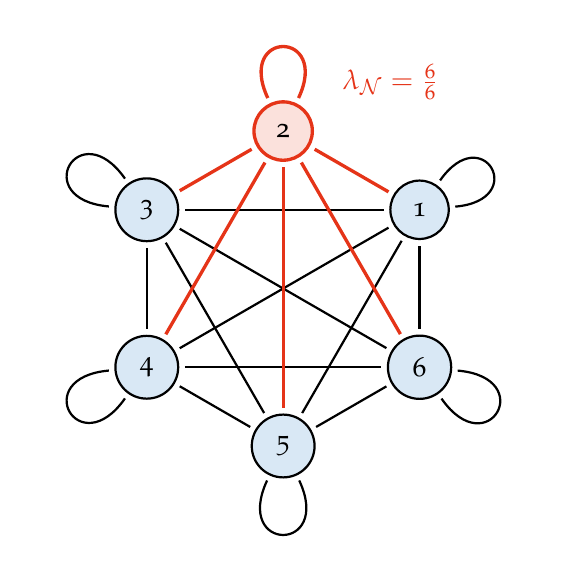
\begin{tikzpicture}
    \tikzstyle{particle} = [draw, circle, fill=tumblue!15, thick, inner sep=5pt];
    \tikzstyle{my loop} = [edge, in=30, out=80, looseness=8, min distance=5mm];

    \foreach \num/\angle in {1/30,3/150,4/210,5/270,6/330} {
        \node[particle] (p\num) at (\angle:2) {\num};
    }
    \foreach \from/\to in {3/4,4/5,5/6,6/1,1/3,1/4,1/5,3/5,3/6,4/6} {
        \draw[edge] (p\from) -- (p\to);
    }
    \foreach \num/\in/\out in {1/5/55,3/125/175,4/185/235,5/245/295,6/305/355} {
        \draw (p\num) edge[loop, my loop, in=\in, out=\out] (p\num);
    }

    \node[particle, marked node] (p2) at (90:2) {2};
    \foreach \from/\to in {2/1,2/3,2/4,2/5,2/6} {
        \draw[edge, marked edge] (p\from) -- (p\to);
    }
    \draw (p2) edge[loop, my loop, in=65, out=115, marked edge] (p2);
    \node[marked, above right=0em and 1em of p2] {$\lambda_\mathcal{N} = \frac{6}{6}$};
\end{tikzpicture}
\end{document}
